\documentclass[11pt]{article}
\usepackage[margin=0.85in]{geometry}
\usepackage{mathptmx} % Times-like font for text and math
\setlength{\parskip}{2pt}
\setlength{\textfloatsep}{6pt}
\setlength{\intextsep}{6pt}
\setlength{\floatsep}{6pt}
\setlength{\abovecaptionskip}{2pt}
\setlength{\belowcaptionskip}{0pt}
\usepackage{amsmath}
\usepackage{amssymb}
\usepackage{booktabs}
\usepackage{graphicx}
\usepackage{float}
\usepackage{hyperref}
\usepackage{array}
\usepackage{xcolor}
\usepackage{enumitem}
\setlist{nosep,leftmargin=*}

\definecolor{highsigma}{RGB}{216,90,48}
\definecolor{lowsigma}{RGB}{29,158,117}
\definecolor{querycol}{RGB}{83,74,183}
\definecolor{lightcoral}{RGB}{250,236,231}
\definecolor{lightteal}{RGB}{225,245,238}

\title{Learning Decision-Focused Embeddings\\for Contextual Stochastic Optimization}
\author{Kaiwen Li \quad Woojin Chae \quad Soochan Kim\\[4pt]
DSO 619 Final Project\\[2pt]
Code and replication materials: \href{https://github.com/checcoli/DSO-619}{\texttt{https://github.com/checcoli/DSO-619}}}
\date{\today}

\begin{document}
\maketitle

\begin{abstract}
Local prescriptors for contextual stochastic optimization---kernel weighted SAA, $k$-NN, decision-focused forests---all depend on an implicit notion of context similarity. We argue that the right object to learn is therefore not a downstream solver but a \emph{decision-focused embedding}: a low-dimensional context representation whose neighborhoods are aligned with the downstream cost rather than with conditional-mean fit. We learn the embedding end-to-end by minimizing prescriptive regret of weighted SAA in the embedded space, then test whether the same embedding transfers as a drop-in replacement for raw features in other prescriptors. Four controlled synthetic benchmarks isolate complementary mechanisms (nuisance-dimension removal, decision-vs-prediction misalignment, boundary alignment, cost-function dependence), and we compare against PCA, LASSO, prediction-trained embeddings, spectral-mixture kernels, neural embeddings, and the official \emph{Stochastic Optimization Forests} (SOF) implementation. The benchmarks show that decision-focused training provides gains beyond generic representation learning, that the learned embedding genuinely depends on the cost function (as the newsvendor service level approaches the tail, the metric reallocates mass from mean-relevant to variance-relevant coordinates), and that the embedding transfers: plugging it into SOF as a drop-in replacement for raw features reduces forest regret from 1.304 to 0.303 on the rotated heteroscedastic benchmark, even though the forest is never retrained jointly with the embedding.
\end{abstract}

%%% ---------------------------------------------------------------
\section{Introduction}\label{sec:intro}
%%% ---------------------------------------------------------------

\paragraph{Problem statement and central research question.}
Contextual stochastic optimization prescribes an action $z$ given a context $x$ and historical data $\{(x_i,y_i)\}_{i=1}^N$. Local prescriptors---weighted SAA~\cite{bertsimas2020predictive}, $k$-NN, decision-focused forests~\cite{kallus2023sof}---all rest on an implicit notion of \emph{which historical contexts are similar to the current query}. In raw feature space, that similarity is decision-blind: it weights every coordinate equally regardless of whether it drives the cost. The central research question of this paper is:
\begin{quote}
\emph{Can we learn a low-dimensional context embedding $\phi:\mathbb R^d\to\mathbb R^{d'}$ such that (i) similarity in the embedded space is aligned with the downstream cost rather than with conditional-mean fit, and (ii) the same embedding transfers as a drop-in input to other prescriptors, decoupling the geometry from the solver?}
\end{quote}
We answer ``yes'' on both fronts through a controlled empirical study. The kernel is used only as a training device for $\phi$; the embedding is the deliverable. Kernel SAA is $O(N^2)$ at training and $O(N)$ per query at inference; decision-focused forests~\cite{kallus2023sof} are much faster but their axis-aligned splits are a poor match to rotated or heteroscedastic decision surfaces. Our approach \emph{decouples the embedding from the prescriptor}: learn $\phi$ via kernel SAA on a small training set, then plug $\phi$ into any downstream solver. Off-the-shelf representation learners (PCA, LASSO, prediction-trained kernel metrics, MSE neural embeddings) target the conditional mean rather than the cost, and need not agree with a decision-focused embedding; end-to-end global methods such as SPO+~\cite{elmachtoub2022smart} and decision-focused networks~\cite{donti2017task,wilder2019melding} learn the policy $x\mapsto z$ directly but forfeit the data efficiency and interpretability of local approaches. Our method bridges the two---local training, transferable geometry.

The experiment suite is organized around five questions. \textbf{Q1}: are the gains from decision-focused training rather than from representation learning in general? \textbf{Q2}: do they come from removing nuisance dimensions? \textbf{Q3}: in the rotated benchmarks, do they come from decision-boundary alignment rather than better prediction fit? \textbf{Q4}: does the learned embedding depend on the cost function? \textbf{Q5}: does $\phi$ transfer to a different prescriptor as a drop-in replacement for raw features? Q5 is arguably the most practically relevant: kernel SAA does not scale, but if $\phi$ transfers to a scalable solver, the scalability limitation is moot. The answer on Benchmark~B is a $4\times$ regret reduction when $\phi_{\mathrm{dec}}$ is plugged into a decision-focused forest. Section~\ref{sec:formulation} formalizes the decision problem; Section~\ref{sec:related} surveys related work; Section~\ref{sec:method} the learning pipeline; Sections~\ref{sec:benchA}--\ref{sec:sof_transfer} the empirical results; Sections~\ref{sec:feedback} and \ref{sec:contributions} the feedback incorporation and author contributions. Supporting examples are in the appendix.

%%% ---------------------------------------------------------------
\section{Problem Formulation}\label{sec:formulation}
%%% ---------------------------------------------------------------

We make the decision problem explicit before introducing any learning machinery. A reader should be able to identify the decision variable, the objective, the constraints, the uncertainty, the timing of information, what is observed at decision time, and what is estimated from data. We then state the auxiliary learning problem we solve to make these decisions, and explain in words how the mathematical objects fit together.

\paragraph{The decision problem.}
At decision time, the planner observes a context $x \in \mathcal X \subseteq \mathbb R^d$ (e.g., the features of an arriving demand signal) but \emph{not} the realization of the uncertain outcome $Y \in \mathcal Y$ (e.g., realized demand or a vector of rewards). She must choose a decision $z \in \mathcal Z$ and then incurs the realized cost $c(z,Y)$. The objective is to minimize the expected cost conditional on the observed context:
\begin{equation}\label{eq:contextual-so}
v^\star(x) \;=\; \min_{z \in \mathcal Z}\; \mathbb E\!\left[\,c(z,Y)\,\bigm|\, X=x\,\right],
\qquad
z^\star(x) \;\in\; \arg\min_{z \in \mathcal Z}\; \mathbb E\!\left[\,c(z,Y)\,\bigm|\, X=x\,\right].
\end{equation}
The components are:
\begin{itemize}
    \item \textbf{Decision variable.} $z \in \mathcal Z$. In our newsvendor benchmarks (A, B, D), $\mathcal Z = \mathbb R_{\ge 0}$ is an order quantity. In the allocation benchmark (C), $\mathcal Z = \{0,1\}$ selects one of two projects.
    \item \textbf{Objective.} $\mathbb E[c(z,Y)\mid X=x]$. For newsvendor at service level $\alpha$, $c_\alpha(z,y)=\alpha\max(y-z,0)+(1-\alpha)\max(z-y,0)$, whose conditional optimizer is the $\alpha$-quantile of $Y\mid X{=}x$. For two-action allocation, $c(z,r)=-r_z$ and the optimizer picks the action with the larger conditional mean reward.
    \item \textbf{Constraints.} The decision must lie in $\mathcal Z$. No additional resource or coupling constraints across queries are imposed in our benchmarks.
    \item \textbf{Uncertainty.} The outcome $Y$ is random with unknown conditional distribution $\mathbb P(Y\mid X{=}x)$. The cost depends on $z$ and the realization of $Y$.
    \item \textbf{Timing.} (i) Historical sample $\{(x_i,y_i)\}_{i=1}^N$ is collected i.i.d.\ from $\mathbb P(X,Y)$; (ii) a context $x$ is revealed at decision time; (iii) the planner commits to $z$; (iv) $Y$ realizes and the cost $c(z,Y)$ is incurred.
    \item \textbf{What is observed at decision time.} Only the context $x$ and the historical sample. The realization $Y$ is \emph{not} observed before $z$ is chosen.
    \item \textbf{What is estimated from data.} The conditional distribution of $Y\mid X{=}x$ is unknown and must be approximated from $\{(x_i,y_i)\}_{i=1}^N$. We approximate it through a set of nonnegative \emph{context weights} $\{w_i(x)\}_{i=1}^N$ with $\sum_i w_i(x)=1$, which place a discrete distribution $\sum_i w_i(x)\delta_{y_i}$ on the historical outcomes.
\end{itemize}

\paragraph{Weighted-SAA prescription.}
Given weights $w_i(x)$, the data-driven prescription is the weighted sample-average approximation of \eqref{eq:contextual-so}:
\begin{equation}\label{eq:wSAA}
\hat z(x;w) \;\in\; \arg\min_{z\in\mathcal Z}\; \sum_{i=1}^N w_i(x)\, c(z,y_i).
\end{equation}
The quality of $\hat z(x;w)$ is measured by \emph{prescriptive regret} relative to the oracle policy $z^\star$ that knows the conditional distribution:
\begin{equation}\label{eq:regret}
R(\hat z) \;=\; \mathbb E_{X}\!\left[\,\mathbb E\bigl[c(\hat z(X;w),Y) - c(z^\star(X),Y)\,\bigm|\, X\bigr]\,\right].
\end{equation}
Regret, not predictive MSE, is the performance metric.

\paragraph{Geometry-induced weights.}
We restrict attention to weights derived from a Gaussian kernel applied in an \emph{embedded} context space:
\begin{equation}\label{eq:kernel-weights}
w_{\phi,h,i}(x) \;=\; \frac{K_h\bigl(\phi(x),\phi(x_i)\bigr)}{\sum_{j=1}^N K_h\bigl(\phi(x),\phi(x_j)\bigr)},
\qquad
K_h(u,u') \;=\; \exp\!\left(-\frac{\|u-u'\|_2^2}{2h^2}\right),
\end{equation}
where $\phi:\mathbb R^d\to\mathbb R^{d'}$ is the learned embedding and $h>0$ is a bandwidth. In words: $\phi$ controls \emph{which historical points are similar to $x$}, and $h$ controls \emph{how localized the neighborhood is}.

\paragraph{The learning problem.}
The embedding $\phi$ is itself estimated from data. Conceptually:
\begin{equation}\label{eq:learning}
\phi_{\mathrm{dec}} \;\in\; \arg\min_{\phi \in \Phi}\;
\mathbb E_{X,Y}\!\left[\,c\bigl(\hat z(X;w_{\phi,h}),\,Y\bigr)\,\right]
\;+\; \lambda\,\Omega(\phi),
\end{equation}
where $\Phi$ is a parametric family (Mahalanobis, neural residual MLP) and $\Omega$ is a regularizer. In practice the expectation is replaced by an empirical leave-one-out decision loss (Section~\ref{sec:method}). A prediction-trained baseline $\phi_{\mathrm{pred}}$ replaces the cost $c$ in \eqref{eq:learning} by squared error against $y$.

\paragraph{Verbal interpretation.}
The mathematical objects fit together as a two-level problem. The \emph{outer} problem chooses an embedding $\phi$, i.e., a geometry over historical contexts. The \emph{inner} problem chooses, for each query $x$, the action $z$ that minimizes a $\phi$-weighted empirical cost over historical outcomes. The downstream solver in \eqref{eq:wSAA} can be replaced---e.g., by a decision-focused forest with leaf-co-occurrence weights---without changing the geometry $\phi$, which is precisely what we test in the embedding-transfer experiment (Q5).

%%% ---------------------------------------------------------------
\section{Related Work}\label{sec:related}
%%% ---------------------------------------------------------------

\paragraph{Weighted SAA and decision-focused forests.}
Bertsimas and Kallus~\cite{bertsimas2020predictive} unify $k$-NN, kernel, tree, and local-linear weights under a single weighted-SAA framework with consistency guarantees. Any consistent weight estimator yields a consistent prescription, but the finite-sample rate deteriorates with ambient dimension---when $x$ enters the value function only through a $k$-dimensional projection with $k\ll d$, a fixed isotropic kernel pays the full ambient rate while a learned embedding can recover the intrinsic rate~\cite{stone1982optimal}. Kallus~\cite{kallus2023sof} extends weighted SAA to \emph{Stochastic Optimization Forests} (SOF), where leaf co-occurrence induces the weights; we use the official implementation as a baseline and as the downstream solver in the transfer experiments.

\paragraph{Decision-focused learning and metric learning.}
SPO+~\cite{elmachtoub2022smart} replaces prediction loss with a regret surrogate for the downstream LP; Donti et al.~\cite{donti2017task} and Wilder et al.~\cite{wilder2019melding} extend end-to-end training to stochastic and combinatorial settings; Liu and Grigas~\cite{liu2021risk} add risk calibration; Mandi et al.~\cite{mandi2024decision} survey the field. All learn a \emph{global} policy $x\mapsto z$. We instead train an \emph{embedding} that feeds a local prescriptor, so $\phi$ is transferable. On the metric-learning side, Lanckriet et al.~\cite{lanckriet2004learning} and G\"onen \& Alpaydin~\cite{gonen2011multiple} learn kernel matrices and MKL combinations for predictive fit; spectral mixture kernels~\cite{wilson2013gaussian} and compositional kernel search~\cite{duvenaud2013structure} extend the form space; Weinberger and Tesauro~\cite{weinberger2007metric} and Bellet et al.~\cite{bellet2013survey} learn Mahalanobis metrics from regression and task-aware losses. TaskMet~\cite{bansal2024taskmet} is closest: it uses task loss to learn a metric that reshapes the \emph{prediction} loss in a predict-then-optimize pipeline; we instead learn a metric in \emph{context} space to determine which observations receive weight in distribution-preserving weighted SAA. Besbes, Ma, and Mouchtaki~\cite{besbes2025contextual} flag estimating the dissimilarity $d$ from data as an open question; our embedding provides one answer.

%%% ---------------------------------------------------------------
\section{Method}\label{sec:method}
%%% ---------------------------------------------------------------

Section~\ref{sec:formulation} introduced kernel-weighted SAA \eqref{eq:wSAA}--\eqref{eq:kernel-weights} and the decision-focused learning problem \eqref{eq:learning}. This section instantiates them. The fixed-kernel baseline sets $\phi=I$ after standardizing features; decision and prediction bandwidths are selected from $\{0.20,0.35,0.50,0.75,1.00,1.50,2.00\}$ times the median pairwise distance in the embedded training set.

\paragraph{Two-stage prediction-first baselines.}
PCA~+~kernel keeps the top $k$ principal components (Benchmark~A only; on the rotated 2D benchmarks PCA is rotation-equivalent to the fixed kernel). LASSO~+~kernel solves $\min_{\beta_0,\beta}\frac{1}{n}\sum_i(y_i-\beta_0-x_i^\top\beta)^2+\lambda\|\beta\|_1$ with $\lambda$ chosen by validation MSE, then runs the fixed kernel on the selected coordinates.

\paragraph{Prediction-trained and decision-trained embeddings (matched family).}
Both train the \emph{same} embedding family on different objectives:
\[
\phi_{\mathrm{pred}} \in \arg\min_\phi \frac{1}{m}\sum_j \bigl(\hat\mu_\phi^{(-j)}(x_j)-y_j\bigr)^2 + \lambda\Omega(\phi),
\qquad
\phi_{\mathrm{dec}} \in \arg\min_\phi \frac{1}{m}\sum_j c\bigl(\hat z_\phi^{(-j)}(x_j),y_j\bigr) + \lambda\Omega(\phi),
\]
where $\hat\mu_\phi^{(-j)}$ is the leave-one-out kernel-regression mean and $\hat z_\phi^{(-j)}$ is the leave-one-out weighted-SAA prescription. In the implementation $\phi_{\mathrm{dec}}$ is initialized at $\phi_{\mathrm{pred}}$ and then fine-tuned on the decision loss, so the Q1 comparison is ``same family, different training objective.'' Because $c$ enters \eqref{eq:learning} explicitly, $\phi_{\mathrm{dec}}$ may depend on the cost---Benchmark~D tests this directly.

\paragraph{Embedding parameterizations.}
We use a screened diagonal Mahalanobis map $\phi(x)=\mathrm{diag}(\sqrt{s_1},\dots,\sqrt{s_d})x$ on Benchmark~A (top 10 features get individual scales, the rest share one nuisance scale; raw $\log s_j$ are mean-centered to remove $(L,h)$ non-identifiability); a rotated anisotropic Mahalanobis $\phi(x)=\mathrm{diag}(\sqrt{s_1},\sqrt{s_2})R(\varphi)x$ on Benchmarks~B and~C; a plain diagonal Mahalanobis on Benchmark~D; and a residual MLP $\phi_\theta(x)=x+W_2\tanh(W_1x+b_1)+b_2$ on Benchmarks~B and~C. All maps are globally shared across queries (no input-dependent $L(x)$).

\paragraph{Official SOF and embedding-aware SOF variants.}
For the newsvendor benchmarks we use the official \emph{Stochastic Optimization Forests}~\cite{kallus2023sof} replication code (the ``rf\_approx\_sol'' variant), with leaf-co-occurrence weights $w_i(x)=T^{-1}\sum_t \mathbf 1\{i\in L_t(x)\}/|L_t(x)|$. The diagnostic hybrid LASSO$\to$SOF first applies the supervised screen and then fits the same forest backend on the retained coordinates. For the transfer experiment (Section~\ref{sec:sof_transfer}) we fix the forest algorithm and vary only the input embedding $g\in\{g_{\mathrm{raw}},g_{\mathrm{PCA}},g_{\mathrm{LASSO}},\phi_{\mathrm{pred}},\phi_{\mathrm{dec}}\}$, yielding SOF-raw, SOF-PCA, SOF-LASSO, SOF-pred, and SOF-dec. Forests are not rotation-invariant, so SOF-PCA is meaningful even where PCA + kernel collapses to the fixed kernel. For the regret decomposition we additionally use leaf-smoothed weights $\bar w_i\propto w_i\exp(-\|\tilde x-\tilde x_i\|^2/2h^2)$.

\paragraph{Prediction MSE diagnostic.}
For Q3, each method receives a \emph{separate} predictive bandwidth chosen by validation MSE against the true conditional mean, decoupling ``bad prediction'' from ``bad decision bandwidth.''

\subsection*{Experimental design}\label{sec:expdesign}

\textbf{Methods compared.} The full slate spans (i)~\emph{Kernel-fixed}, (ii)~\emph{PCA~+~kernel}, (iii)~\emph{LASSO~+~kernel}, (iv)~\emph{Kernel-pred}, (v)~\emph{Kernel-dec}, (vi)~\emph{Spectral-mixture kernel}, (vii)~\emph{Neural embedding}, (viii)~\emph{Official SOF}, (ix)~\emph{LASSO$\to$SOF}, and (x)~\emph{Embedding-aware SOF variants}. \textbf{Why they are appropriate.} The fixed kernel quantifies the cost of not learning geometry. PCA and LASSO are the canonical two-stage (``reduce, then prescribe'') answers and isolate variance-based and prediction-based screening. Kernel-pred matches Kernel-dec in embedding family and differs only in training objective---the tightest test of decision-vs-prediction misalignment. Official SOF is the leading decision-focused forest and provides the alternative way to obtain decision-aware local weights. SOF plug-ins isolate the contribution of $\phi$ from the contribution of the downstream solver. \textbf{Metrics.} Primary: prescriptive regret \eqref{eq:regret} averaged over replications, computed against the closed-form oracle of each synthetic DGP. Secondary: out-of-sample predictive MSE against the true conditional mean (Q3 diagnostic). For Benchmark~D we also report the $x_2$-mass share of the diagonal Mahalanobis. \textbf{What each benchmark teaches.} \emph{A} (Q2): sparse axis-aligned nuisance regime, tests dimension removal. \emph{B} (Q1,~Q3): rotated heteroscedastic newsvendor, tests recovery of variance directions invisible to MSE. \emph{C} (Q3): rotated piecewise allocation boundary, tests decision-boundary alignment without nuisance or heteroscedasticity. \emph{D} (Q4): newsvendor with $\alpha$ swept and the DGP held fixed, tests cost-dependence of the embedding. \emph{Transfer} (Q5): fixes the forest algorithm and varies only $\phi$, testing whether the embedding is reusable across prescriptors.

%%% ---------------------------------------------------------------
\section{Benchmark A: Nuisance Removal (Q2)}\label{sec:benchA}
%%% ---------------------------------------------------------------
\subsection*{Data-generating process}
Benchmark A isolates the nuisance-feature mechanism. Contexts satisfy
\[
X=(U,V), \quad U\in\mathbb R^k,\quad V\in\mathbb R^{d-k},
\]
with all coordinates i.i.d.\ $\mathcal N(0,1)$ and only $U$ affecting demand: $Y\mid X\sim \mathcal N(25+\beta^\top U,\,4^2)$ with $\beta_j\ne 0$ only for $j\le k$. Newsvendor costs $(c_u,c_o)=(4,1)$ give target quantile $\alpha=0.8$. Homoscedastic Gaussian noise aligns the decision target with the conditional mean up to a shift, so this benchmark isolates nuisance-dimension removal rather than decision-vs-prediction misalignment. Equal marginal variance also makes the PCA comparison especially sharp: PCA has no population-level information about which directions are decision-relevant, so the benchmark is intentionally hostile to variance-based reduction while still fair to response-aware screening (LASSO). We sweep $d\in\{5,10,20,50,100\}$, $k\in\{1,3,5\}$, $N\in\{100,200,400,800\}$ with six replications per configuration.

\subsection*{Results}
\begin{table}[H]
\centering
\small
\resizebox{\textwidth}{!}{%
\begin{tabular}{lrrrrrrrrrrrrr}
\toprule
$d$ & $k$ & Fixed & PCA & LASSO & Pred.-trained repr. & Decision-trained repr. & SOF & LASSO$\to$SOF & LASSO signal share & Pred. signal mass & Decision signal mass & SOF signal split & LASSO$\to$SOF split \\
\midrule
5.0 & 1.0 & 1.233 & 4.147 & 0.699 & 0.329 & 0.439 & 0.375 & 0.392 & 0.61 & 0.83 & 0.74 & 0.35 & 0.68 \\
5.0 & 3.0 & 1.634 & 3.664 & 1.473 & 1.025 & 1.130 & 1.007 & 0.987 & 0.69 & 0.93 & 0.94 & 0.78 & 0.82 \\
5.0 & 5.0 & 2.193 & 2.193 & 2.193 & 1.942 & 2.119 & 2.681 & 2.681 & 1.00 & 1.00 & 1.00 & 1.00 & 1.00 \\
10.0 & 1.0 & 2.172 & 4.094 & 1.068 & 0.365 & 0.478 & 0.339 & 0.345 & 0.36 & 0.73 & 0.64 & 0.26 & 0.47 \\
10.0 & 3.0 & 2.754 & 5.120 & 1.735 & 1.127 & 1.180 & 1.142 & 1.049 & 0.61 & 0.74 & 0.71 & 0.59 & 0.77 \\
10.0 & 5.0 & 3.882 & 5.578 & 3.105 & 2.247 & 2.450 & 2.890 & 2.773 & 0.72 & 0.92 & 0.87 & 0.76 & 0.87 \\
20.0 & 1.0 & 2.974 & 4.545 & 1.037 & 0.456 & 0.438 & 0.305 & 0.318 & 0.29 & 0.57 & 0.62 & 0.23 & 0.43 \\
20.0 & 3.0 & 3.539 & 5.203 & 2.571 & 1.230 & 1.154 & 1.113 & 0.997 & 0.31 & 0.73 & 0.74 & 0.46 & 0.59 \\
20.0 & 5.0 & 5.100 & 7.229 & 3.616 & 2.143 & 2.331 & 3.020 & 2.731 & 0.54 & 0.83 & 0.81 & 0.58 & 0.77 \\
50.0 & 1.0 & 3.447 & 4.497 & 1.796 & 0.341 & 0.382 & 0.439 & 0.419 & 0.28 & 0.50 & 0.51 & 0.17 & 0.41 \\
50.0 & 3.0 & 4.648 & 6.006 & 2.685 & 1.178 & 1.204 & 1.261 & 1.006 & 0.35 & 0.75 & 0.78 & 0.34 & 0.59 \\
50.0 & 5.0 & 6.815 & 8.374 & 4.901 & 2.465 & 2.481 & 3.552 & 3.123 & 0.32 & 0.70 & 0.69 & 0.41 & 0.62 \\
100.0 & 1.0 & 3.846 & 4.570 & 1.429 & 0.272 & 0.283 & 0.440 & 0.354 & 0.26 & 0.71 & 0.67 & 0.16 & 0.40 \\
100.0 & 3.0 & 5.111 & 5.888 & 2.784 & 1.119 & 1.252 & 1.511 & 1.090 & 0.37 & 0.60 & 0.59 & 0.28 & 0.61 \\
100.0 & 5.0 & 7.144 & 8.162 & 4.764 & 3.228 & 3.379 & 3.737 & 3.119 & 0.36 & 0.66 & 0.68 & 0.34 & 0.63 \\
\bottomrule
\end{tabular}

}
\caption{Benchmark A regret snapshot at $N=400$ together with each supervised reducer's emphasis on the true signal block. For learned metrics, this is diagonal mass share; for SOF and LASSO$\to$SOF, it is split-frequency share.}
\label{tab:benchmark_a_snapshot}
\end{table}

The benchmark confirms the nuisance-removal mechanism. PCA fails uniformly: with all coordinates of equal marginal variance, it has no information about which block carries signal, and its effective exponents are essentially zero. Supervised reduction helps substantially: at $(d,k,N)=(20,3,400)$, regret falls from 3.539 (fixed kernel) to 2.571 (LASSO~+~kernel), 1.230 ($\phi_{\mathrm{pred}}$), and 1.154 ($\phi_{\mathrm{dec}}$). The official SOF baseline is genuinely competitive on this axis-aligned sparse benchmark: it reaches 1.113 at the same setting, and LASSO$\to$SOF improves to 0.997; across the 60-configuration grid, SOF beats LASSO in 56 cases and LASSO$\to$SOF further improves on SOF in 47. Feature-emphasis at $(20,3,400)$ tracks the mechanism cleanly---signal-share is $0.31$ (LASSO), $0.73$ ($\phi_{\mathrm{pred}}$), $0.74$ ($\phi_{\mathrm{dec}}$), $0.46$ (SOF), $0.59$ (LASSO$\to$SOF). Continuous metric learning remains highly competitive, especially in the largest ambient dimensions, but A alone does not establish that metric learning is uniquely responsible for nuisance removal---the forest's axis-aligned bias is also well matched here. The effective-exponent table and signal-block importance plot are in Appendix~\ref{app:extra_figs}.

%%% ---------------------------------------------------------------
\section{Benchmark B: Decision-vs-Prediction Misalignment (Q1, Q3)}\label{sec:benchB}
%%% ---------------------------------------------------------------
\subsection*{Data-generating process}
Define rotated coordinates $u=\cos(\pi/4)x_1+\sin(\pi/4)x_2$ and $v=-\sin(\pi/4)x_1+\cos(\pi/4)x_2$. The conditional mean depends only on $u$, $\mu(x)=25+8\tanh(2u)$; the conditional sd depends on both, $\sigma(x)=2(0.8+1.2\,\mathbf 1\{v>0\}+0.2|u|)$; and $Y\mid X=\mu(x)+\sigma(x)\varepsilon$ with $\varepsilon\sim\mathcal N(0,1)$. For the $\alpha=0.8$ newsvendor, the oracle order is $q^\star(x)=\mu(x)+\sigma(x)\Phi^{-1}(0.8)$. A mean-MSE-trained embedding has incentive to recover $u$ but not $v$, since $v$ affects variance not mean; the quantile decision depends on both, so a decision-focused embedding must learn $v$ as well. This is the Q1/Q3 separation.

\subsection*{Results}
\begin{table}[H]
\centering
\small
\begin{tabular}{lrrr}
\toprule
Method & Avg. cost & Avg. regret & Avg. pred. MSE \\
\midrule
Global SAA & 9.832 & 5.459 & 40.995 \\
Point prediction & 8.336 & 3.963 & 6.843 \\
Fixed kernel & 5.146 & 0.774 & 1.689 \\
LASSO + kernel & 5.146 & 0.774 & 1.689 \\
Pred.-trained repr. & 4.862 & 0.490 & 0.746 \\
Decision-trained repr. & 4.799 & 0.426 & 1.003 \\
Spectral mixture & 5.220 & 0.848 & 1.971 \\
Neural embedding & 4.777 & 0.405 & 1.134 \\
SOF & 5.294 & 0.922 & 3.655 \\
LASSO$\to$SOF & 5.295 & 0.923 & 3.651 \\
\bottomrule
\end{tabular}

\caption{Benchmark B summary over 20 replications. PCA is omitted because, in 2D, keeping both PCs is equivalent to the fixed kernel.}
\label{tab:benchmark_b_summary}
\end{table}

Two-stage screening does not rescue this benchmark: LASSO~+~kernel and LASSO$\to$SOF match the fixed kernel and SOF respectively because LASSO selects both raw coordinates in all 20 replications. SOF reaches average regret 0.922 with predictive MSE 3.655; the screened hybrid is statistically indistinguishable (0.923 / 3.651). Both forest variants are far better than point-prediction but worse than the fixed kernel, and much worse than the learned embeddings. Average regret falls from 0.774 (fixed kernel) to 0.490 ($\phi_{\mathrm{pred}}$) and 0.426 ($\phi_{\mathrm{dec}}$); the decision-trained method beats the prediction-trained baseline in 15/20 replications. \emph{The matched Mahalanobis comparison is the primary Q1 evidence:} the prediction-trained embedding has lower conditional-mean MSE (0.746 vs.\ 1.003) but higher regret (0.490 vs.\ 0.426). The spectral mixture kernel underperforms; the neural embedding is best at 0.405 regret, though its conditional-mean MSE is still worse than $\phi_{\mathrm{pred}}$'s. The forest weakness is structural: an axis-aligned partition is a poor match to the rotated heteroscedastic decision surface, and there are no nuisance dimensions for the supervised screen to remove.

%%% ---------------------------------------------------------------
\section{Benchmark C: Boundary Alignment in Resource Allocation (Q3)}\label{sec:benchC}
%%% ---------------------------------------------------------------
\subsection*{Data-generating process}
Two-action allocation $\mathcal Z=\{0,1\}$ with latent boundary $u=\cos(\pi/4)x_1+\sin(\pi/4)x_2$. The projects swap dominance at $u=0$: $\mathbb E[R_0\mid x]=12+0.4u$ if $u>0$ else $5+0.4u$, and $\mathbb E[R_1\mid x]$ symmetrically. Observed rewards add i.i.d.\ $\mathcal N(0,2.5^2)$ noise; the prescriptor picks the action with the larger weighted empirical reward.

\subsection*{Results}
\begin{table}[H]
\centering
\small
\begin{tabular}{lrrr}
\toprule
Method & Avg. cost & Avg. regret & Avg. pred. MSE \\
\midrule
Global SAA & -8.466 & 3.853 & 14.682 \\
Point prediction & -12.135 & 0.184 & 4.555 \\
Fixed kernel & -12.126 & 0.193 & 2.139 \\
Pred.-trained repr. & -12.209 & 0.109 & 1.194 \\
Decision-trained repr. & -12.213 & 0.106 & 1.467 \\
Spectral mixture & -12.146 & 0.173 & 2.052 \\
Neural embedding & -12.247 & 0.072 & 0.696 \\
LASSO$\to$SOF & -12.008 & 0.311 & 1.993 \\
\bottomrule
\end{tabular}

\caption{Benchmark C summary over 20 replications.}
\label{tab:benchmark_c_summary}
\end{table}

Within the primary Mahalanobis family, the Q3 result persists: regret falls from 0.109 to 0.106 after decision-focused fine-tuning while reward-vector MSE worsens from 1.194 to 1.467. The spectral mixture kernel again underperforms (0.173 vs.\ fixed kernel 0.193). The diagnostic LASSO$\to$SOF is poor (regret 0.311, MSE 1.993, worse than even the fixed kernel); multi-output LASSO keeps both coordinates in all 20 replications, so screening cannot blame the result on unremoved nuisance. The neural embedding wins clearly at 0.072 regret and 0.696 MSE, and the boundary slice (Appendix~\ref{app:extra_figs}, Fig.~\ref{fig:benchmark_c_summary}) shows it tracks the oracle transition most sharply near $u=0$, where regret is concentrated.

%%% ---------------------------------------------------------------
\section{Benchmark D: Cost-Dependent Embedding (Q4)}\label{sec:benchD}
%%% ---------------------------------------------------------------

\subsection*{Setup}
Benchmarks~A--C show that $\phi_{\mathrm{dec}}$ can beat $\phi_{\mathrm{pred}}$ at a \emph{fixed} cost. A stricter test is whether the learned embedding actually \emph{depends on} the cost. We vary only the service level $\alpha$ while holding the DGP fixed: $X=(x_1,x_2)$ are i.i.d.\ $\mathcal N(0,1)$, $Y\mid X=\beta x_1+\exp(\gamma x_2)\varepsilon$ with $\beta=3$, $\gamma=1.2$, $\varepsilon\sim\mathcal N(0,1)$, so the mean signal is $\beta x_1$ and the multiplicative noise scale $\exp(\gamma x_2)$ spans roughly two orders of magnitude. The newsvendor cost is $c_\alpha(z,y)=\alpha\max(y-z,0)+(1-\alpha)\max(z-y,0)$ and the oracle order is $q^\star_\alpha(x)=\beta x_1+\exp(\gamma x_2)\Phi^{-1}(\alpha)$: at $\alpha=0.5$ only $x_1$ matters; as $\alpha\to 1$, $x_2$ becomes increasingly decision-relevant. A prediction-trained embedding emphasizes $x_1$ regardless of $\alpha$; a decision-trained one has incentive to weight $x_2$ at the tail. We sweep $\alpha\in\{0.50,0.70,0.85,0.90,0.95,0.99\}$ with 20 replications ($N_{\mathrm{tr}}=250$, $N_{\mathrm{val}}=150$, $N_{\mathrm{te}}=2000$) using the diagonal Mahalanobis $\phi(x)=\mathrm{diag}(\sqrt{s_1},\sqrt{s_2})x$ and report the $x_2$-share $s_2/(s_1+s_2)$. $\phi_{\mathrm{pred}}$ is fit once per replication; $\phi_{\mathrm{dec}}$ is refit per $\alpha$ via grid search + Powell refinement.

\subsection*{Results}
\begin{table}[H]
\centering
\small
\begin{tabular}{cccccc}
\toprule
$\alpha$ & median pred.\ $x_2$-share & median dec.\ $x_2$-share & mean dec.\ $x_2$-share & pred.\ regret & dec.\ regret \\
\midrule
0.50 & 0.012 & 0.003 & 0.004 & 0.059 & 0.031 \\
0.70 & 0.012 & 0.005 & 0.005 & 0.119 & 0.104 \\
0.85 & 0.012 & 0.021 & 0.038 & 0.196 & 0.164 \\
0.90 & 0.012 & 0.133 & 0.192 & 0.221 & 0.149 \\
0.95 & 0.012 & 0.376 & 0.379 & 0.227 & 0.147 \\
0.99 & 0.012 & 0.609 & 0.580 & 0.161 & 0.101 \\
\bottomrule
\end{tabular}
\caption{Benchmark D summary across $\alpha$, over 20 replications. ``$x_2$-share'' is the diagonal Mahalanobis mass on the variance-relevant coordinate. $\phi_{\mathrm{pred}}$ is $\alpha$-independent by construction (its objective does not see $\alpha$); $\phi_{\mathrm{dec}}$ is refit per $\alpha$ and its median $x_2$-share rises from $0.003$ at $\alpha=0.5$ to $0.609$ at $\alpha=0.99$ even though the DGP is unchanged.}
\label{tab:benchmark_d_summary}
\end{table}

The prediction-trained embedding does not see $\alpha$: a single $\phi_{\mathrm{pred}}$ is fit per replication and reused across the sweep, with median $x_2$-share $0.012$ (correctly identifying $x_1$ as mean-relevant). The decision-trained embedding tracks the cost function: as $\alpha$ moves from $0.5$ to $0.99$, the median $x_2$-share of $\phi_{\mathrm{dec}}$ rises from $0.003$ to $0.609$. At $\alpha=0.5$ the optimizer is the median, which equals $\beta x_1$ under symmetric noise, and $\phi_{\mathrm{dec}}$ correctly ignores $x_2$; at $\alpha\to 1$ the cost weights the upper tail, where $\exp(\gamma x_2)$ dominates, and the embedding shifts mass onto $x_2$. The shift materializes as a real reduction in prescriptive cost: at $\alpha=0.95$ regrets are $0.227$ ($\phi_{\mathrm{pred}}$) vs.\ $0.147$ ($\phi_{\mathrm{dec}}$); at $\alpha=0.99$, $0.161$ vs.\ $0.101$. (A minority ($\sim$20\%) of replications place $\phi_{\mathrm{pred}}$ in a variance-reduction basin where it weights $x_2$ heavily; this inflates cross-seed variance but cannot couple $\phi_{\mathrm{pred}}$ to $\alpha$, since the prediction objective never sees the cost. Medians are reported.) Because the DGP is held fixed across the sweep, the embedding shift cannot be attributed to a change in the response distribution: decision-blind methods on $(X,Y)$ pairs have no mechanism to produce different embeddings for different cost functions, while $\phi_{\mathrm{dec}}$ does so automatically.

\paragraph{Why SOF helps on A but not on B or C.}
SOF's strength on A is structural: sparse axis-aligned nuisance-removal is its home regime, and LASSO$\to$SOF further removes irrelevant split coordinates upfront. B and C are different: both are constructed around latent $45^\circ$-rotated coordinates, so axis-aligned splits must approximate a rotated decision surface with a staircase, and supervised screening can change nothing because LASSO keeps both coordinates in all 20 replications. The remaining issue is therefore the forest's local geometry, not the screen.

%%% ---------------------------------------------------------------
\section{Embedding Transfer Across Prescriptors (Q5)}\label{sec:sof_transfer}
%%% ---------------------------------------------------------------

Sections~\ref{sec:benchA}--\ref{sec:benchD} learn $\phi$ by optimizing weighted-SAA regret and evaluate it within weighted SAA. The objection is that $\phi$ might be over-fit to the kernel solver's idiosyncrasies. Q5 fixes a \emph{different} prescriptor---a decision-focused forest---and only swaps its input features for $\phi$. \textbf{Apples-to-apples data protocol.} For every benchmark and replication, all methods share \emph{one} training set and one validation set, with no extra split between the embedding stage and the forest stage. Embeddings are fit by leave-one-out within the training set; the SOF forest is then grown on $\{(\phi(x_i),y_i)\}_{i=1}^N$ from the same training set; PCA/LASSO maps for SOF-PCA/SOF-LASSO are also fit on it; validation bandwidths use the held-out set, matching the SOF replication protocol. SOF-pred uses a response-based split criterion on a decision-focused embedding (decision-blind downstream, decision-focused upstream); SOF-dec combines $\phi_{\mathrm{dec}}$ with the official decision-aware impurity.

\subsection*{Results: Benchmarks B and C (rotated regimes)}
We pair methods so the contribution of $\phi$ reads off as a vertical drop within each downstream solver: SOF-raw vs.\ Kernel-fixed; SOF-pred vs.\ Kernel-pred; SOF-dec vs.\ Kernel-dec.

\begin{table}[H]
\centering
\footnotesize
\setlength{\tabcolsep}{4pt}
\begin{tabular}{lrrrrrr}
\toprule
Method & B regret & B MSE & B wins & C regret & C MSE & C wins \\
\midrule
SOF-raw & 1.304 & 5.683 & 0 & 0.324 & 2.221 & 0 \\
SOF-PCA & 0.338 & 0.620 & 20 & 0.058 & 0.470 & 20 \\
SOF-LASSO & 1.326 & 5.778 & 6 & 0.330 & 2.184 & 9 \\
SOF-pred & 0.339 & 0.687 & 20 & 0.082 & 0.563 & 20 \\
SOF-dec & 0.303 & 0.846 & 20 & 0.096 & 0.696 & 20 \\
Kernel-fixed & 0.774 & 1.689 & 20 & 0.193 & 2.139 & 20 \\
Kernel-dec & 0.426 & 1.003 & 20 & 0.106 & 1.467 & 20 \\
Neural-dec & 0.405 & 1.134 & 20 & 0.072 & 0.696 & 20 \\
\bottomrule
\end{tabular}

\caption{Embedding-aware SOF summary on Benchmarks B and C: average regret, predictive MSE, and number of replications (out of 20) that beat SOF-raw.}
\label{tab:benchmark_bc_plugin}
\end{table}

Benchmark~B delivers a strong transfer result: average regret drops from 1.304 (SOF-raw) to 0.339 (SOF-pred) and 0.303 (SOF-dec), even though the forest objective is unchanged. The comparison is genuinely decision-focused: SOF-dec beats SOF-pred on regret despite worse predictive MSE (0.846 vs.\ 0.687), reproducing within the transferred-embedding family the prediction-vs-decision separation seen in kernel SAA. Benchmark~C supports transfer but not a universal ranking: SOF-raw 0.324, SOF-PCA 0.058, SOF-pred 0.082, SOF-dec 0.096---geometry matters, but a simple orthogonal reparameterization captures most of the gain on this boundary problem.

A $2\times 2$ decomposition (raw vs.\ decision split) $\times$ (uniform vs.\ kernel-smoothed leaf weights) shows that metric alignment is the first-order effect: SOF-raw$\to$SOF-dec moves $1.304\to 0.303$ on B and $0.324\to 0.096$ on C. Leaf-weight smoothing is secondary---helping the raw-space forest, giving a small further gain on C ($0.096\to 0.083$), but slightly worsening SOF-dec on B ($0.303\to 0.321$). Benchmark-A plug-in diagnostics and the decomposition figures are in Appendix~\ref{app:extra_figs}.

Once fit, $\phi$ is a $d\times d$ Mahalanobis matrix or a residual MLP with $O(d\,d')$ per-query inference cost; the $O(N)$ neighbor scan that limits kernel SAA is a property of the kernel solver, not of the embedding. Decoupling the two---learning $\phi$ via kernel SAA, then handing it to a scalable solver---is the version we expect to be most useful in practice.

%%% ---------------------------------------------------------------
\section{Discussion and Conclusions}\label{sec:conclusions}
%%% ---------------------------------------------------------------

The benchmark suite returns crisp answers to Q1--Q5. \emph{Q1:} the gain is genuinely decision-focused---on Benchmark~B, LASSO~+~kernel collapses to the fixed kernel, official SOF and LASSO$\to$SOF reach 0.922 / 0.923, and within the matched Mahalanobis family the prediction-trained embedding has lower predictive MSE but higher regret than the decision-trained one. \emph{Q2:} the nuisance-removal mechanism is real---in Benchmark~A's sparse axis-aligned regime PCA fails, LASSO helps, official SOF is strong, and LASSO$\to$SOF often improves on SOF; the learned metric is competitive but not uniquely responsible. \emph{Q3:} decision-focused fine-tuning lowers regret while worsening predictive MSE on both B and C, and the neural embedding lowers regret further on the nonlinear benchmarks. \emph{Q4:} Benchmark~D varies only $\alpha$ and the decision-trained embedding shifts mass onto the variance-relevant coordinate, accompanied by a real regret reduction---a behavior no decision-blind method on $(X,Y)$ pairs can reproduce. \emph{Q5:} plugging $\phi_{\mathrm{dec}}$ into SOF on Benchmark~B cuts forest regret $4\times$ ($1.304\to 0.303$) without joint retraining; transfer holds on C but the ranking depends on the benchmark, and on A it is weaker because the forest's native bias is already well aligned. Across the suite the consistent message is that \emph{the right object to learn is the embedding}: it responds to the cost function, transfers across prescriptors (decision-blind and decision-focused alike), and can be paired with scalable solvers at $O(d\,d')$ per-query inference cost.

\textbf{Limitations and future work.} We do not study real-world deployments, locally-adaptive metrics $x\mapsto L(x)x$, or end-to-end training of $\phi$ with the downstream forest. A natural extension is to harvest $\phi$ from the penultimate layer of a directly-trained neural policy $\pi_\theta:x\mapsto z$---particularly useful in higher dimensions where the Mahalanobis family becomes too rigid.

%%% ---------------------------------------------------------------
\section{Response to Presentation and Code-Review Feedback}\label{sec:feedback}
%%% ---------------------------------------------------------------

\textbf{Presentation feedback.} The feedback reshaped the report along three lines, with one headline scope request and several clarity items. (i)~\emph{Framing and positioning.} We revised the title and the opening of Section~\ref{sec:intro} to lead with ``decision-focused embedding / dimensionality reduction'' and explicit ML keywords, rather than a weighted-SAA / Bertsimas--Kallus opener; we also rebuilt Section~\ref{sec:sof_transfer} around the suggested positioning that $\phi$ is the deliverable and the kernel is only a training device, so $\phi$ can be passed to a more scalable downstream DFL solver (Benchmark~B regret falls from $1.304$ for SOF-raw to $0.303$ for SOF-dec). (ii)~\emph{Cost-dependent example---the headline scope request.} The feedback specifically asked for an example where the right embedding actually depends on the downstream cost, since otherwise decision-blind methods would also benefit from rotation/nuisance removal. This produced Benchmark~D (Section~\ref{sec:benchD}): the newsvendor service level $\alpha$ is swept while the DGP is held fixed, and the $x_2$-mass of $\phi_{\mathrm{dec}}$ rises from $0.003$ at $\alpha=0.5$ to $0.609$ at $\alpha=0.99$. This is the part of the paper most directly a response to feedback. (iii)~\emph{Clarity of the transferable-representations material} (called out as the hardest section to follow): methods are now spelled out and grouped into matched pairs (SOF-raw vs.\ Kernel-fixed, SOF-pred vs.\ Kernel-pred, SOF-dec vs.\ Kernel-dec); the apples-to-apples data protocol in Section~\ref{sec:sof_transfer} makes explicit that every method on every replication uses the \emph{same} training and validation set; Section~\ref{sec:sof_transfer} confirms that $\phi$ helps both decision-blind and decision-focused downstream solvers; and the axis-aligned-interpretation question ($Lx$ vs.\ $L_\theta(x)\,x$) is resolved in Section~\ref{sec:method}---all parametric families use a globally shared $\phi$, never an input-dependent $L_\theta(x)$. The stretch suggestion (harvest features from a direct-policy network) is acknowledged in Section~\ref{sec:conclusions} as future work; a full empirical comparison was deferred because it would require a separate policy pipeline and is orthogonal to Q1--Q5.

\textbf{Code-review feedback.} The reviewers raised two items on architecture and maintainability, both addressed in the released repository. (i)~\emph{Explicit replication settings.} The reviewers asked for clearer documentation of benchmark parameters and the SOF-transfer protocol. We added a dedicated \emph{Replication Settings} section to \texttt{README.md} that tables Benchmark~A's full parameter grid ($d\in\{5,10,20,50,100\}$, $k\in\{1,3,5\}$, $N\in\{100,200,400,800\}$, six replications per cell), documents the twenty-replication counts for Benchmarks~B and~C, spells out the \texttt{EXPERIMENT\_PROFILE} fast/full toggle including which cached artifacts correspond to which profile, and explains seed management and cache behaviour, so the experimental setup can be audited without reading source. (ii)~\emph{Performance via vectorization.} A second suggestion was to vectorize \texttt{.iterrows()} loops (specifically in \texttt{build\_existing\_row\_lookup()} in \texttt{experiment\_suite.py}). We profiled the pipeline and found this function accounts for $<0.1\%$ of runtime; the actual bottlenecks are SOF hyperparameter grid search (9--36 forest fits per replication), the Mahalanobis/representation metric learning (many \texttt{minimize()} calls with LASSO grid fitting), and the official 500-tree SOF fits themselves. Vectorizing the lookup would yield $<1\%$ speedup, so we kept the more readable \texttt{.iterrows()} form and instead expose runtime control through the \texttt{EXPERIMENT\_PROFILE} environment variable, which affects the grid-search granularity that dominates total time.

%%% ---------------------------------------------------------------
\section{Author Contributions}\label{sec:contributions}
%%% ---------------------------------------------------------------

Following the CRediT convention, individual contributions are summarized below. All authors reviewed the final manuscript and incorporated the presentation and code-review feedback summarized in Section~\ref{sec:feedback}.
\begin{itemize}
    \item \textbf{Kaiwen Li}: conceptualization and methodology---developed the decision-focused embedding formulation, designed the Q1--Q5 experimental structure, and specified the weighted-SAA learning objective, matched-family baselines, and embedding-transfer protocol; software---built the core kernel-SAA training pipeline and the four synthetic DGPs; formal analysis and investigation---ran the benchmark sweeps, hyperparameter selection, and the $2\times 2$ regret decomposition; co-led writing of the original draft.
    \item \textbf{Woojin Chae}: methodology---co-developed the rotated and cost-dependent benchmark designs and contributed key ideas on the prediction-vs-decision separation; literature review---surveyed the decision-focused-learning, kernel/metric-learning, and finite-sample-theory literatures that inform Section~\ref{sec:related}; software and data curation---debugged and hardened the SOF replication integration and several DGP routines; \emph{led the code review}, producing the architecture and maintainability feedback addressed in Section~\ref{sec:feedback}.
    \item \textbf{Soochan Kim}: experiment design---contributed to the design of Benchmarks~A--D and the embedding-transfer protocol, including the matched-pair pairing of vanilla and embedding-aware variants; visualization---prepared the figures and tables across the empirical sections and the appendix, including the regret curves, feature-emphasis plots, and embedding-transfer diagnostics.
\end{itemize}
Replication code and random seeds are at \href{https://github.com/checcoli/DSO-619}{\texttt{github.com/checcoli/DSO-619}}.

%%% ---------------------------------------------------------------
\begin{thebibliography}{20}

\bibitem{bansal2024taskmet}
D.~Bansal, R.~T.~Q.~Chen, M.~Mukadam, and B.~Amos.
\newblock TaskMet: Task-driven metric learning for model learning.
\newblock In \emph{Advances in Neural Information Processing Systems}, volume~36, 2024.

\bibitem{bellet2013survey}
A.~Bellet, A.~Habrard, and M.~Sebban.
\newblock A survey on metric learning for feature vectors and structured data.
\newblock \emph{arXiv preprint arXiv:1306.6709}, 2013.

\bibitem{bertsimas2020predictive}
D.~Bertsimas and N.~Kallus.
\newblock From predictive to prescriptive analytics.
\newblock \emph{Management Science}, 66(3):1025--1044, 2020.

\bibitem{besbes2025contextual}
O.~Besbes, W.~Ma, and O.~Mouchtaki.
\newblock From contextual data to newsvendor decisions: On the actual
  performance of data-driven algorithms.
\newblock \emph{arXiv preprint arXiv:2302.08424}, 2025.

\bibitem{donti2017task}
P.~L.~Donti, B.~Amos, and J.~Z.~Kolter.
\newblock Task-based end-to-end model learning in stochastic optimization.
\newblock In \emph{Advances in Neural Information Processing Systems}, volume~30, 2017.

\bibitem{duvenaud2013structure}
D.~Duvenaud, J.~R.~Lloyd, R.~Grosse, J.~B.~Tenenbaum, and Z.~Ghahramani.
\newblock Structure discovery in nonparametric regression through compositional kernel search.
\newblock In \emph{Proceedings of the 30th International Conference on Machine Learning}, 2013.

\bibitem{elmachtoub2022smart}
A.~N.~Elmachtoub and P.~Grigas.
\newblock Smart ``predict, then optimize.''
\newblock \emph{Management Science}, 68(1):9--26, 2022.

\bibitem{gonen2011multiple}
M.~G\"onen and E.~Alpaydin.
\newblock Multiple kernel learning algorithms.
\newblock \emph{Journal of Machine Learning Research}, 12:2211--2268, 2011.

\bibitem{kallus2023sof}
N.~Kallus.
\newblock Stochastic optimization forests.
\newblock \emph{Management Science}, 69(4):1975--1994, 2023.

\bibitem{lanckriet2004learning}
G.~R.~G.~Lanckriet, N.~Cristianini, P.~Bartlett, L.~El~Ghaoui, and M.~I.~Jordan.
\newblock Learning the kernel matrix with semidefinite programming.
\newblock \emph{Journal of Machine Learning Research}, 5:27--72, 2004.

\bibitem{liu2021risk}
H.~Liu and P.~Grigas.
\newblock Risk bounds and calibration for a smart predict-then-optimize method.
\newblock In \emph{Advances in Neural Information Processing Systems}, volume~34, pages 19234--19246, 2021.

\bibitem{mandi2024decision}
J.~Mandi, J.~Kotary, S.~Berden, M.~Mulamba, V.~Bucarey, T.~Guns, and F.~Fioretto.
\newblock Decision-focused learning: Foundations, state of the art, benchmark and future opportunities.
\newblock \emph{Journal of Artificial Intelligence Research}, 80:1623--1701, 2024.

\bibitem{stone1982optimal}
C.~J.~Stone.
\newblock Optimal global rates of convergence for nonparametric regression.
\newblock \emph{The Annals of Statistics}, 10(4):1040--1053, 1982.

\bibitem{weinberger2007metric}
K.~Q.~Weinberger and G.~Tesauro.
\newblock Metric learning for kernel regression.
\newblock In \emph{Proceedings of the 11th International Conference on Artificial Intelligence and Statistics}, PMLR 2:612--619, 2007.

\bibitem{wilder2019melding}
B.~Wilder, B.~Dilkina, and M.~Tambe.
\newblock Melding the data-decisions pipeline: Decision-focused learning for combinatorial optimization.
\newblock In \emph{Proceedings of the AAAI Conference on Artificial Intelligence}, volume~33, pages 1658--1665, 2019.

\bibitem{wilson2013gaussian}
A.~G.~Wilson and R.~P.~Adams.
\newblock Gaussian process kernels for pattern discovery and extrapolation.
\newblock In \emph{Proceedings of the 30th International Conference on Machine Learning}, 2013.

\end{thebibliography}

%%% ---------------------------------------------------------------
\appendix
\section{Additional Figures and Tables}\label{app:extra_figs}

This appendix collects supporting diagnostics referenced from the main text.

\begin{figure}[H]
\centering
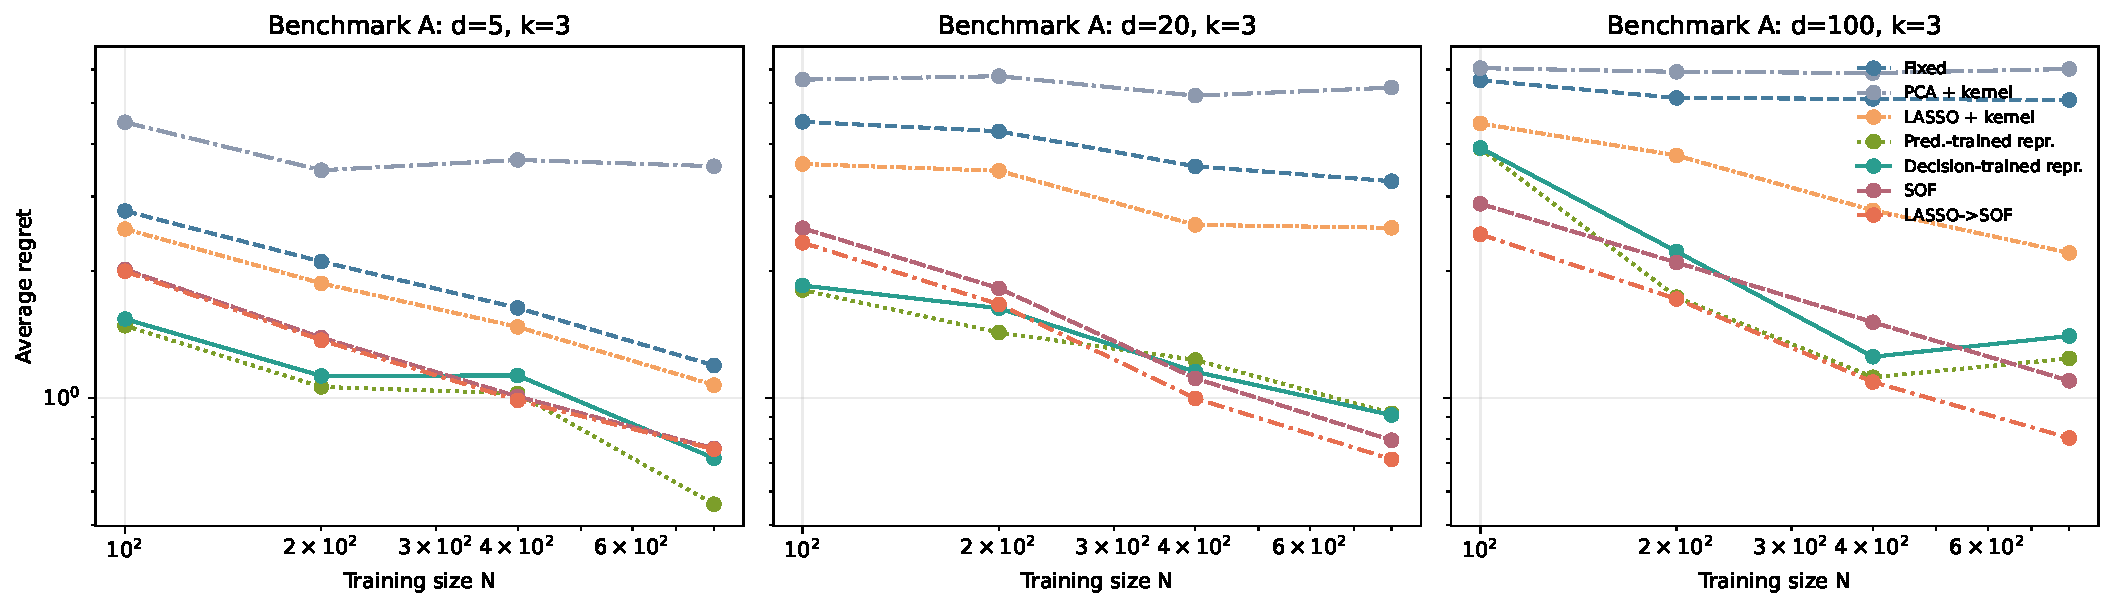
\includegraphics[width=0.90\textwidth]{assets/figures/benchmark_a_loglog_k3.pdf}
\caption{Benchmark A log-log regret curves for representative $k=3$ settings. PCA fails because variance directions are uninformative; supervised screening helps; and both SOF-style tree neighborhoods and learned metrics improve once nuisance dimensions dominate.}
\end{figure}

\begin{figure}[H]
\centering
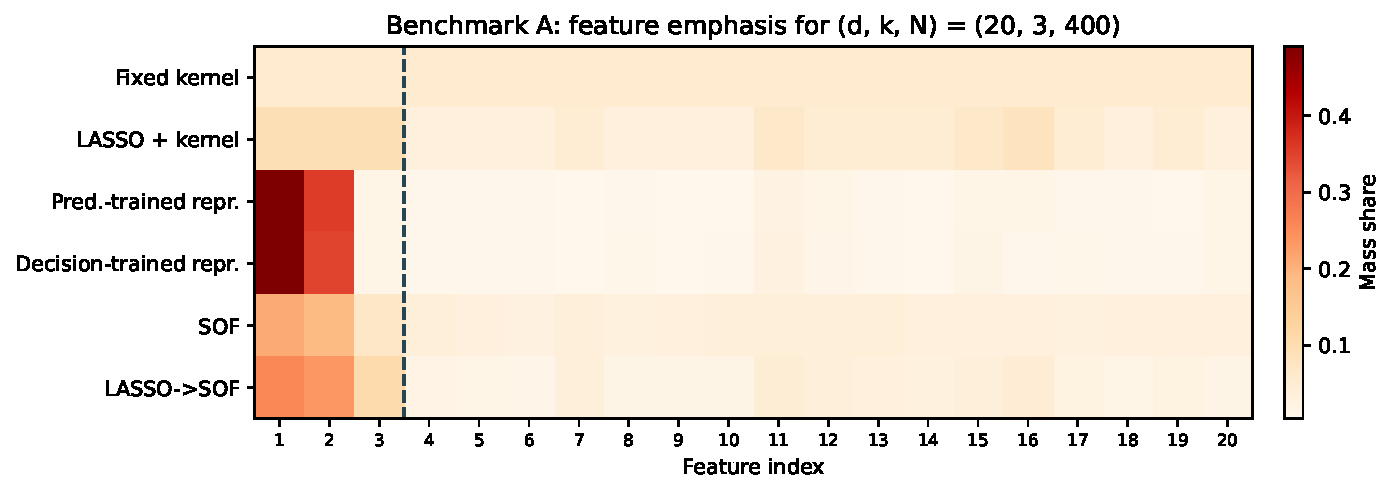
\includegraphics[width=0.85\textwidth]{assets/figures/benchmark_a_importance.pdf}
\caption{Benchmark A feature emphasis for the representative setting $(d,k,N)=(20,3,400)$. The dashed line separates the true signal block from nuisance coordinates. For SOF and LASSO$\to$SOF the emphasis is split-frequency share rather than metric mass.}
\end{figure}

\begin{table}[H]
\centering
\small
\begin{tabular}{lrrrrrrrr}
\toprule
$d$ & $k$ & Fixed & PCA & LASSO & Pred.-trained repr. & Decision-trained repr. & SOF & LASSO$\to$SOF \\
\midrule
5.0 & 1.0 & 0.43 & 0.02 & 0.91 & 0.80 & 0.71 & 0.63 & 0.47 \\
5.0 & 3.0 & 0.40 & 0.10 & 0.40 & 0.43 & 0.33 & 0.47 & 0.47 \\
5.0 & 5.0 & 0.40 & 0.40 & 0.40 & 0.34 & 0.31 & 0.42 & 0.42 \\
10.0 & 1.0 & 0.25 & 0.03 & 0.56 & 0.36 & 0.29 & 0.68 & 0.56 \\
10.0 & 3.0 & 0.27 & 0.02 & 0.31 & 0.40 & 0.35 & 0.51 & 0.52 \\
10.0 & 5.0 & 0.25 & 0.10 & 0.29 & 0.30 & 0.31 & 0.35 & 0.36 \\
20.0 & 1.0 & 0.15 & 0.02 & 0.47 & 0.36 & 0.51 & 0.57 & 0.54 \\
20.0 & 3.0 & 0.17 & 0.03 & 0.19 & 0.31 & 0.36 & 0.57 & 0.59 \\
20.0 & 5.0 & 0.13 & -0.01 & 0.15 & 0.31 & 0.29 & 0.30 & 0.31 \\
50.0 & 1.0 & 0.09 & 0.01 & 0.32 & 0.45 & 0.44 & 0.55 & 0.42 \\
50.0 & 3.0 & 0.12 & 0.03 & 0.26 & 0.46 & 0.51 & 0.48 & 0.52 \\
50.0 & 5.0 & 0.07 & 0.02 & 0.16 & 0.20 & 0.22 & 0.33 & 0.36 \\
100.0 & 1.0 & 0.05 & 0.02 & 0.61 & 1.10 & 1.15 & 0.59 & 0.51 \\
100.0 & 3.0 & 0.05 & 0.00 & 0.35 & 0.56 & 0.53 & 0.46 & 0.55 \\
100.0 & 5.0 & 0.05 & 0.01 & 0.12 & 0.46 & 0.42 & 0.31 & 0.32 \\
\bottomrule
\end{tabular}

\caption{Benchmark A effective exponents across the full method grid. Larger exponents indicate faster regret decay.}
\label{tab:benchmark_a_exponents}
\end{table}

\begin{figure}[H]
\centering
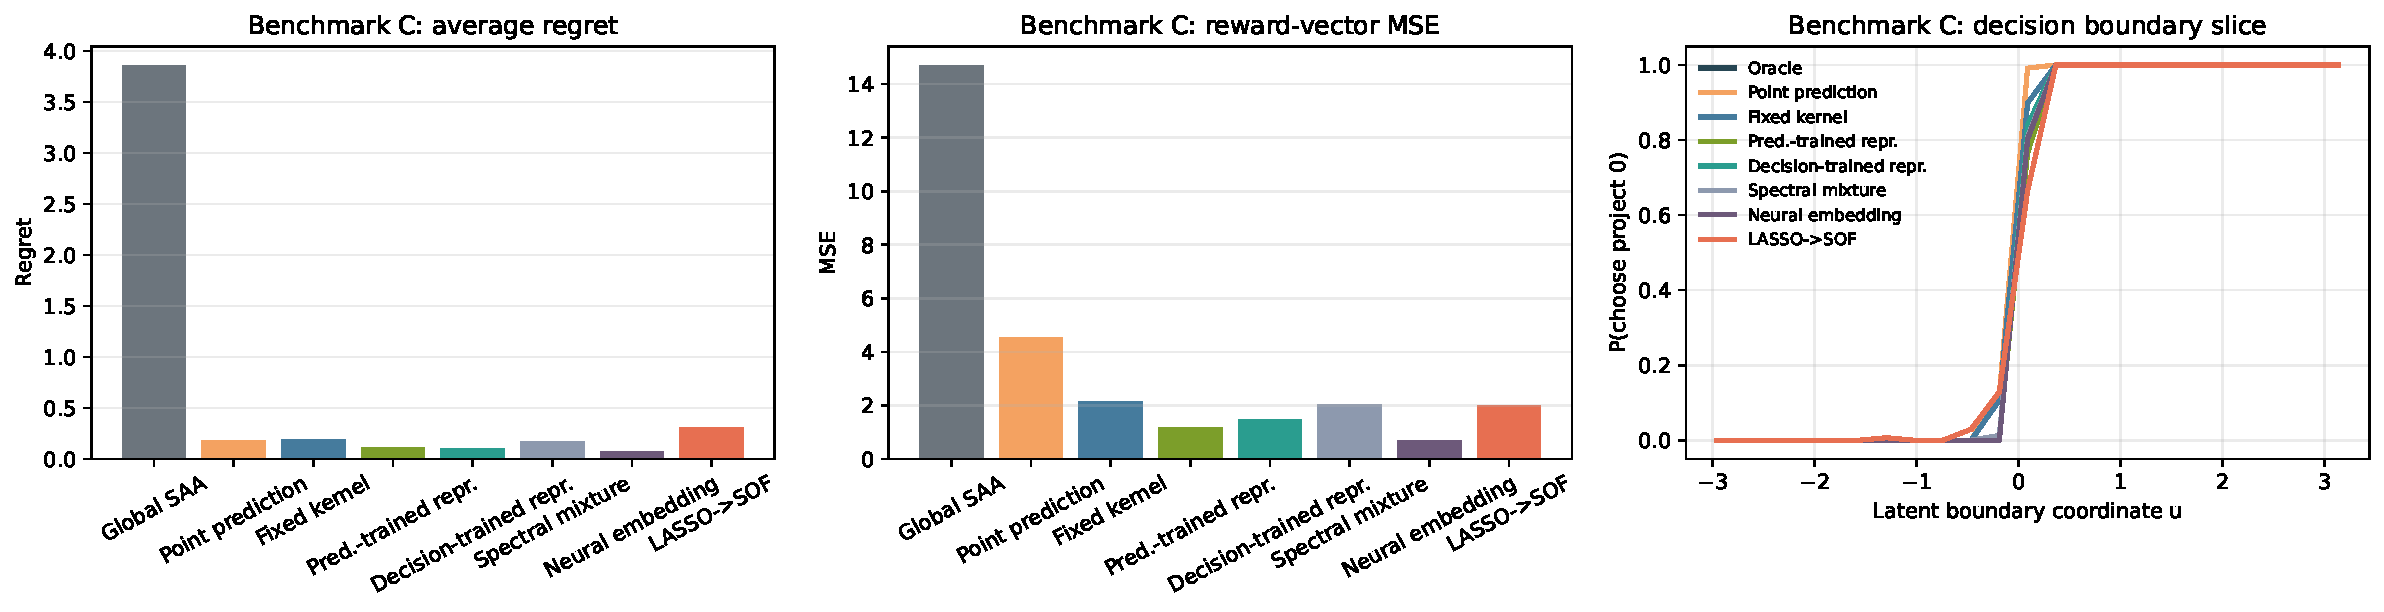
\includegraphics[width=0.95\textwidth]{assets/figures/benchmark_c_summary.pdf}
\caption{Benchmark C. Left: average regret. Middle: reward-vector MSE. Right: probability of choosing project 0 as a function of the latent boundary coordinate $u$. The neural curve tracks the oracle transition most sharply near $u=0$.}
\label{fig:benchmark_c_summary}
\end{figure}

\begin{figure}[H]
\centering
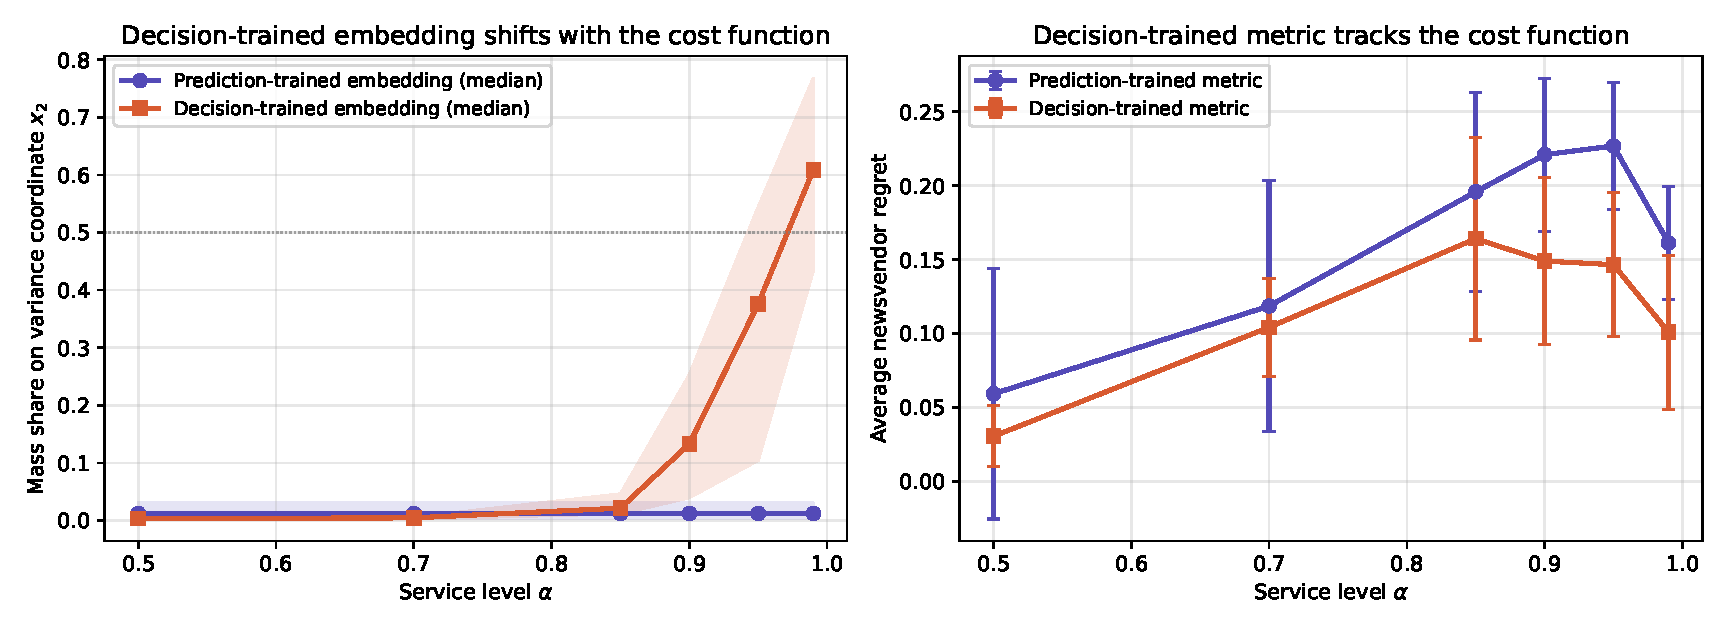
\includegraphics[width=0.95\textwidth]{assets/figures/service_level_summary.pdf}
\caption{Benchmark D. Left: variance-coordinate mass share of the learned diagonal Mahalanobis embedding as a function of $\alpha$ (median over 20 replications, shaded band is the $25$\textendash$75$\% range). The prediction-trained curve is flat (its objective does not see $\alpha$); the decision-trained curve rises monotonically. Right: out-of-sample newsvendor regret. The decision-trained embedding matches or beats the prediction-trained baseline at every $\alpha$, with the gap widening at the tail.}
\label{fig:benchmark_d_summary}
\end{figure}

\begin{figure}[H]
\centering
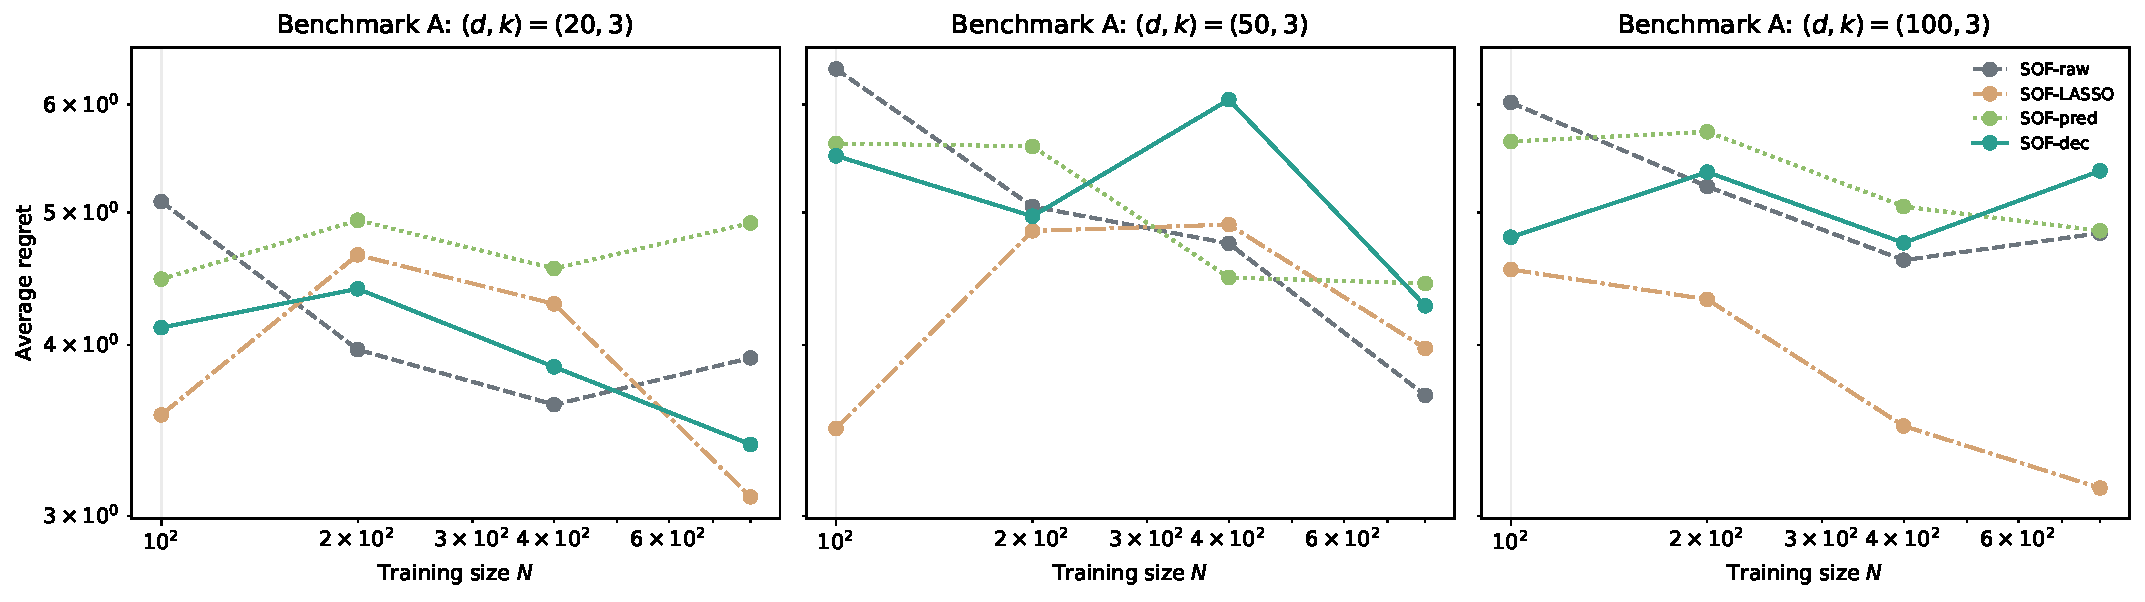
\includegraphics[width=0.85\textwidth]{assets/figures/benchmark_a_plugin_sof_loglog.pdf}
\caption{Benchmark A plug-in SOF regret curves for the representative settings $(d,k)=(20,3),(50,3),(100,3)$. In this axis-aligned sparse regime, SOF-LASSO is the most reliable plug-in baseline; SOF-pred and SOF-dec are less stable.}
\end{figure}

\begin{figure}[H]
\centering
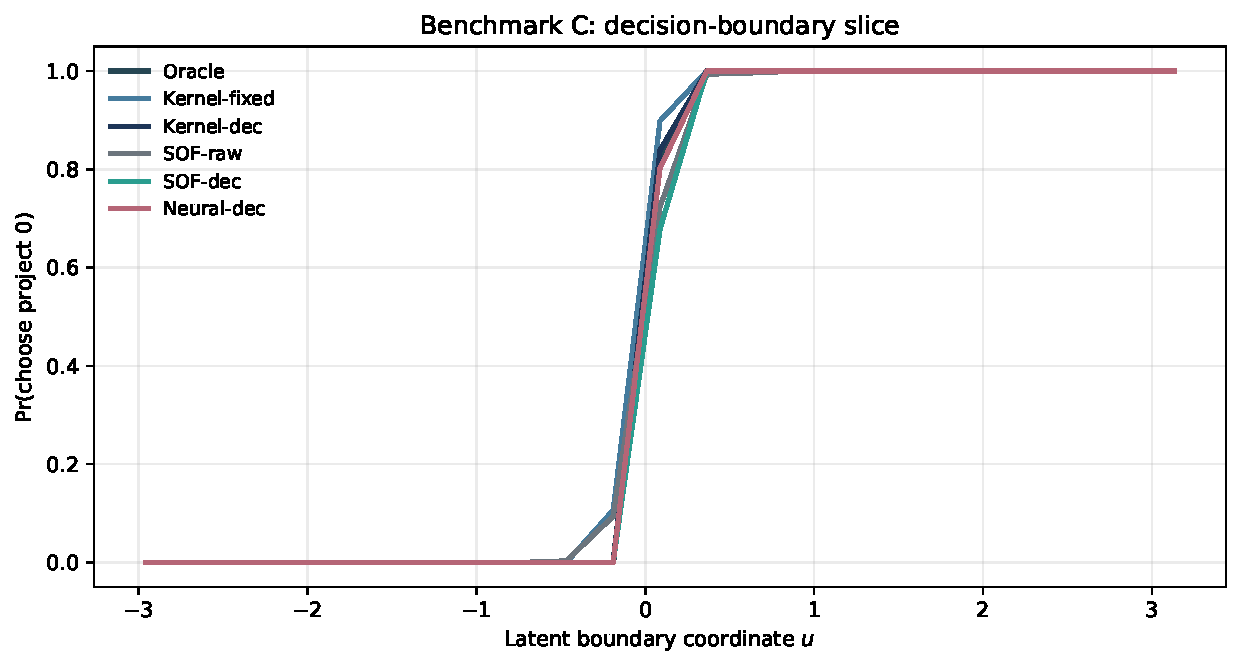
\includegraphics[width=0.85\textwidth]{assets/figures/benchmark_c_plugin_boundary.pdf}
\caption{Benchmark C decision-boundary slice for the plug-in SOF comparison. The transferred embeddings move the forest's transition region much closer to the oracle boundary near $u=0$.}
\end{figure}

\begin{figure}[H]
\centering
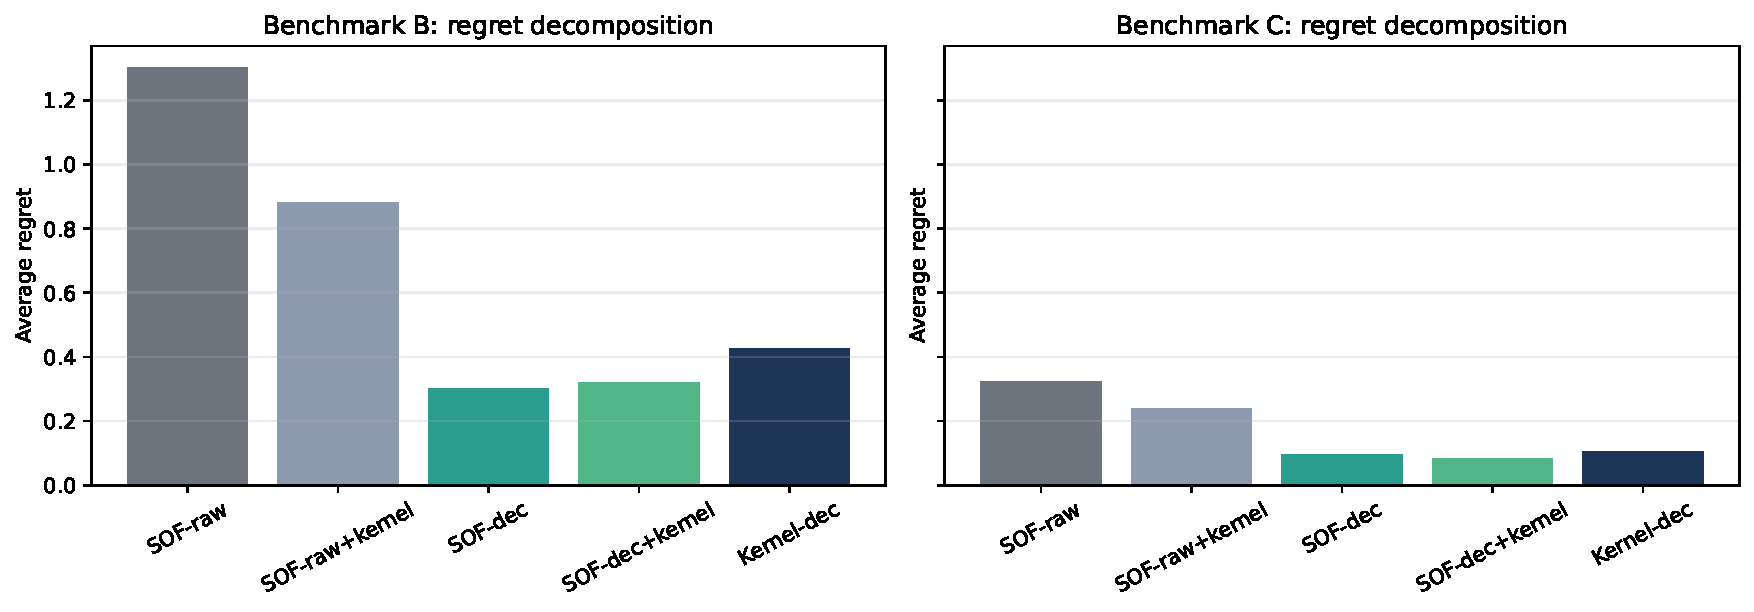
\includegraphics[width=0.92\textwidth]{assets/figures/benchmark_bc_decomposition.pdf}
\caption{Regret decomposition on Benchmarks B and C. The dominant drop comes from moving the forest into the decision-relevant embedding space; leaf-level kernel smoothing has a smaller and benchmark-dependent effect.}
\end{figure}

\end{document}
